\newchap{Experiments: Data Collection and Preprocessing}
\label{chap:data_collection}
The first practical part of this thesis is concerned with data collection. Although phonetics is an important sub-area in linguistics, phonetic transcriptions are hard to find. If there are any transcriptions available, there are various hindrances that prevent it from being used as is. In the following, I outline the different data types which are available and the different strategies that are used to convert the data into one well-formatted corpus. There is quite a famous set of phonetic texts which is a collection of short stories called \textit{The North Wind and the Sun}. Those stories were the starting point for my search for data. The reason for this is that the short stories are available in many different languages. As the corpus  this thesis is based on is a large multilingual corpus, the availability of data in many languages was one of the key criteria to look choose the datasets.

One of the first things I have noticed while collecting my datasets is the abundance of different codes and names to refer to the languages. I have decided to us the ISO 396-3 convention, not to be confused with the ISO 396-2 convention which uses sometimes completely different codes and does not cover all of my languages. ISO 396-3 distinguishes some more dialects and variants. This also means that throughout my research I paid close attention to what variant was actually referred to. For some cases, it seems that there exists a dataset for a language which is in the 100LC, but actually it is not the same variant. To make sure I pick the same code and language, I used the Glottolog as reference\myfootnote{https://glottolog.org/glottolog}.


\section{Transcription sources \& formats}
Phonetic transcriptions of various languages are available from different sources in different formats. From what I have found out in my research phonetic transcriptions are available as either full texts or a word lists.

\subparagraph{Full Text}
For the task of \ac{g2p} conversion, phonetic transcriptions in the form of fully transcribed texts would be ideal. As became clear, it is hardly possible to find those. There is plenty of material describing how different languages can be transcribed but those rarely contain fully transcribed text. If they do, it is mostly limited to one or a few sentences. Additionally, some texts include short descriptions where certain pronunciations rules are explained which are not included in the transcriptions (especially stress). Apart from \ac{nws} short texts described in section, there are no full texts available in multiple languages that could be used.

\subparagraph{Pronunciation Dictionaries}
Another data type that is found quite often are word lists. Those are sometimes referred to as pronunciation dictionaries. However, these often mean that there are words mapped to an audio representation which is not what is meant in this present case. Pronunciation dictionary in this present case refers to the mapping of an orthographic word to its pronunciation using phonetic symbols. Although such lists are very handy, especially as they can easily be used to train a transcription model, transcriptions of individual words and of entire texts are not exactly the same. There are two major problems:

\begin{itemize}
\item Pronunciation depends on the context of the word in question. Word forms are ambiguous and sometimes their pronunciation differs given on their specific context. 
\item Phonetic boundaries are not always equivalent with word boundaries. Spoken language sometimes merges certain words which leads to one phonetic unit.
\end{itemize} 

Data in the form of word lists can be found quite a lot when compare to the availability of full text. An example is the Nidaba\myfootnote{\url{http://nidaba.co.uk/Contents/OriginalWordList}} website that presents a few word lists in different languages. What becomes clear when looking at this data is that there are two important limitations: First, there are only very few languages available that are in my corpus. Second, there are different transcription conventions used.

\subparagraph{Transcription conventions}
No matter how the transcriptions are formatted, a crucial factor is the transcription convention. The \ac{ipalpha} is a well-known convention but there is a lot of data that is available using a different convention. Although it might be possible to convert one convention into another convention this is very tedious and often those conventions are made specifically for one language or a group of related languages. 

\tab{tab:all_langs}{In this table I list all languages that I am using for my experiments.}{
\begin{tabularx}{\textwidth}{|Xll >{\raggedright}rl|}
\hline
\textbf{Iso 639-3} & \textbf{Language name}  & \textbf{Type WikiPron} & \textbf{\# Words WikiPron} & \textbf{Type NWS} \\ \hline
\hline
cmn                & Chinese                 & broad                  & 133,686                    & unk               \\
deu                & German                  & broad                  & 34,145                     & broad             \\
deu                & German                  & narrow                 & 10,984                     & narrow            \\
ell                & Greek (Modern)          & broad                  & 10,547                     & unk               \\
eng                & English US              & broad                  & 57,230                     & broad             \\
eng                & English US              & narrow                 & 1,633                      & narrow            \\
eng                & English UK              & broad                  & 60,422                     & -                 \\
eng                & English UK              & narrow                 & 1,284                      & -                 \\
eus                & Basque (Goizueta)       & broad                  & 1,742                      & broad             \\
fin                & Finnish                 & broad                  & 69,015                     & -                 \\
fin                & Finnish                 & narrow                 & 69,008                     & -                 \\
fra                & French                  & broad                  & 56,911                     & unk               \\
hin                & Hindi                   & narrow                 & 9,563                      & -                 \\
hin                & Hindi                   & broad                  & 10,812                     & unk               \\
ind                & Indonesian              & broad                  & 1,555                      & unk               \\
ind                & Indonesian              & narrow                 & 2,637                      & -                 \\
jpn                & Japanese (Hiragana)     & narrow                 & 19,689                     & -                 \\
kat                & Georgian                & broad                  & 15,123                     & broad             \\
kor                & Korean                  & narrow                 & 14,141                     & unk               \\
mya                & Burmese                 & broad                  & 4,631                      & broad             \\
rus                & Russian                 & narrow                 & 402,586                    & unk               \\
spa                & Spanish (Castilian)     & broad                  & 60,677                     & broad             \\
spa                & Spanish (Castilian)     & narrow                 & 52,190                     & narrow            \\
spa                & Spanish (Latin America) & broad                  & 48,649                     & -                 \\
spa                & Spanish (Latin America) & narrow                 & 41,845                     & -                 \\
tgl                & Tagalog                 & broad                  & 3,321                      & -                 \\
tgl                & Tagalog                 & narrow                 & 1,915                      & -                 \\
tha                & Thai                    & broad                  & 15,050                     & unk               \\
tur                & Turkish                 & broad                  & 1,789                      & unk               \\
tur                & Turkish                 & narrow                 & 1,812                      & -                 \\
vie                & Vietnamese              & narrow                 & 15,240                     & unk               \\
zul                & Zulu                    & broad                  & 1,677                      & -                 \\ \hline
\end{tabularx}}{Languages for experiments}

\section{The 100 language corpus}
\label{sec:corpus}
The basis of the data used in this thesis is a corpus provided by the SPUR lab at the \ac{uzh}. The text group of the Language and Space lab at the University of Zurich maintains a project that provides a multilingual corpus consisting of 100 language text samples \citep{UniversityofZurich.19.07.2021} which is referred to as 100LC (see section \ref{sec:corpus}). Those 100 languages are meant to be representative for all the world's languages. It is therefore meant to give insight on relations, similarities, differences or properties of individual languages or language families. Specifically, their goal is to use quantitative methods like statistical modelling, machine learning and information theory to study language variation and compare languages. The corpus contains 100 languages which are proposed by \citet{Comrie&Dryer.2013}. This is an online book that contains different chapters each of which shows a different linguistic feature including a map which shows the distribution of that feature over the world's languages. While the number of languages presented on the individual maps depends on the amount of research done in a specific area, the sum of all maps gives quite an impressive overview on the structure of nearly half of the world's languages. Out of the 2676 languages a sample of 100 languages was chosen. This sample does not contain too many languages from one area, neither does it contain too many languages from one family. Those are the 100 languages that are in the corpus. Not considering the aforementioned criteria of maximizing genealogical and areal diversity can lead to misleading results in multilingual analysis. Figure \ref{fig:100lc} shows the distribution of the corpus on a world map. The different icons show the genus of the languages which is a classification of languages defined by the \ac{wals} team that maintains the language description collection. The interactive map can be viewed online \citep{100LC.21.07.2021}. Table \ref{tab:100LC} in the appendix A shows all languages that are in the 100 language corpus. None of the text samples are provided by \ac{wals}. The entire corpus is provided by the SPUR team that collected the corpus over the last few years and is continuously working on and with it.

\fig{images/100sample.png}{fig:100lc}{WALS - Map that shows the 100 Languages}{\textwidth}{100 Language Map}

\begin{figure}[h]
\vspace*{-1.5cm}
    \begin{center}
    \hspace*{-2cm}
      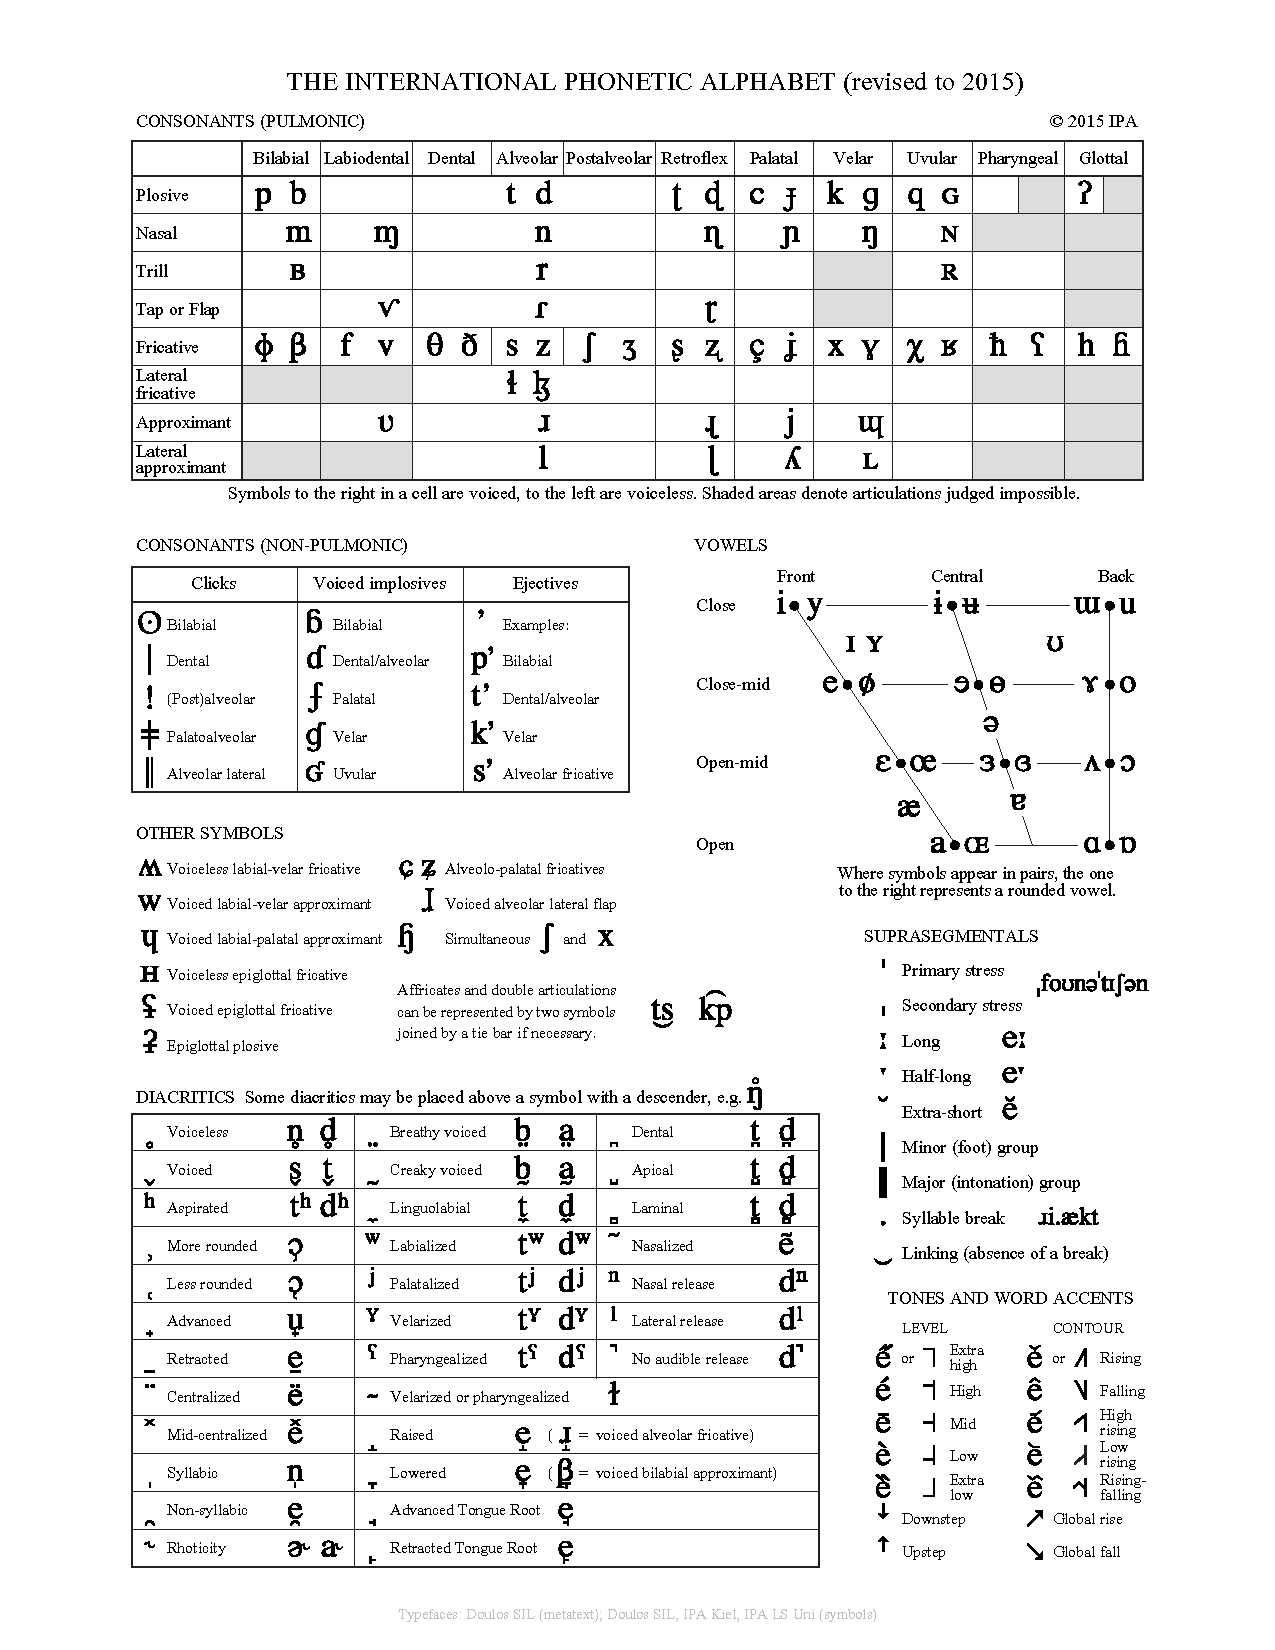
\includegraphics[width=1.3\linewidth]{ipa_chart.pdf}
    \end{center}
    \stepcounter{myfigure}
    \caption[Full IPA chart]{This is the full IPA chart, last updated in 2015}
    \label{fig:ipa_chart}
  \end{figure}


\section{Data used for this thesis}
\label{sec:dataset}
Based on the outcome of my research on the availability of phonetic data, I decided to use two datasets for my experiments in this thesis. I will introduce both of them below. 

\subsection{WikiPron}
A very recent project that publishes pronunciation lists is WikiPron. The WikiPron project \citep{Lee&Ashby.2020} is an open-source Python mining tool to retrieve pronunciation data from Wiktionary. Their database contains 1.7 million word/pronunciation pairs in 165 languages. Both, the database and the tool, are freely available online. Apart from the mining tool and the database, WikiPron can be used for grapheme-to-phoneme modelling. The WikiPron data for one language is always structured the same. It is a tsv-file that has graphemes as a first column and corresponding phonemes as the second column. While the graphemes are just listed as-is, the phonemes are split using the segments library which I shortly presented in section \ref{sec:unicode_ipa}. The phoneme segments are separated by white spaces. 
The WikiPron data has already been used in shared tasks which means that results on this data can easily be compared to other results. For a shared task in 2021 organized by \ac{sigm}, the WikiPron data was improved and additional scripts were added based on feedback and findings from a similar task in 2020. One major improvement was concerned with languages written in different scripts. WikiPron supports now the detection of different scripts and languages can be sorted according to those scripts. For some languages, there is a filtered version of either the broad or the narrow transcription available. Whenever possible, I used this one.


\subsection{The North Wind and the Sun}
\label{nws}
Quite a well-known phonetic corpus is a collection of short stories. The \ac{jpa} continuously published different phonetic transcriptions of a short story called \textit{The North Wind and the Sun}. The story is a fable said to be written by Aesop and has been translated into many languages. Additionally, for many languages there exits a phonetic transcription. As I have mentioned before, many of these texts are available already transcribed and free to use \citep{GitHub.04.02.2022}. Table \ref{north-wind-stories} shows the languages for which the short story is available and which are also in the 100 language corpus. \citet{baird_evans_greenhill_2021} performed an analysis on these texts to find out how many tokens we need to cover a phonetic inventory of a language adequately. What they have found out in their study is that those short stories are by far not long enough to give a good picture of the phonetics of a language. This is of course problematic if those texts are used to demonstrate how a language works phonetically. That said, I will use these stories with care and only as an additional dataset to have more variety.

\tab{tab:north-wind-stories}{ The table shows a list of all the short stories \textit{The North Wind and the
Sun} that are available as phonetic text and whose languages are in the 100
language corpus.}{
\begin{tabular}{|llll|}
\hline
\textbf{Iso 639-3} & \textbf{Type}    & \textbf{Variation} & \textbf{Language} \\
\hline
\hline
arn      & broad and narrow &              & Mapudungun       \\
cmn      &                  & Pekinese     & Mandarin Chinese \\
deu      & broad and narrow & North German & German           \\
ell      &                  &              & Modern Greek     \\
eng      & broad and narrow & Americsn     & English          \\
eus      & broad and narrow & Goizueta     & Basque           \\
hau      & narrow           &              & Hausa            \\
heb      &                  &              & Modern Hebrew    \\
hin      & narrow           &              & Hindi            \\
ind      &                  &              & Indonesian       \\
kat      & broad and narrow &              & Georgian         \\
kor      &                  &              & Korean           \\
mya      &                  &              & Burmese          \\
pes      &                  &              & Western Farsi    \\
spa      & broad and narrow & Castilian    & Spanish          \\
tha      &                  &              & Thai             \\
tur      & broad            & Istanbul     & Turkish          \\
\hline       
\end{tabular}
}{Overview NWS stories}

Below, I include the English version of the short story. 

\begin{quote}
The North Wind and the Sun were disputing which was the stronger, when a traveler came along wrapped in a warm cloak. They agreed that the one who first succeeded in making the traveler take his cloak off should be considered stronger than the other. Then the North Wind blew as hard as he could, but the more he blew the more closely did the traveler fold his cloak around him; and at last the North Wind gave up the attempt. Then the Sun shined out warmly, and immediately the traveler took off his cloak. And so the North Wind was obliged to confess that the Sun was the stronger of the two.
\end{quote}

\subsubsection{Transcription of NWS stories}
A collection of the \ac{nws} stories is available in a handbook of the \ac{jpa} which is only available as a pdf scan of the original book \citep{JIPA2010}. Luckily, most of those texts have been transcribed and made available by Simon Greenhill \citep{GitHub.04.02.2022}. At least the phonetic part of it, the original version was still not available already transcribed. Before I knew about the availability of these texts, I did some research on \ac{ocr} for \ac{ipalpha} texts and manual transcription. While \ac{ocr} is technically possible it turns out to be very difficult for IPA characters. There are tools that include \ac{ipalpha} character recognition like the ABBYY FineReader which can be acquired for a fee. The CL institute at the \ac{uzh} owns a version of the ABBYY tool but this version does not include the IPA module. I ran the ABBYY version on a \ac{jpa} pdf containing said phonetic transcriptions but the result could not be used. Mostly diacritics and special phonetic symbols were not correctly transcribed. These are exactly those characters that make it difficult to transcribe \ac{ipalpha} manually, so there is not point in using this tool. There are also open source tools. One of which is called tesseract. tesseract does not include the IPA alphabet. It is possible to train the model to include the IPA alphabet but this would need appropriate training data\myfootnote{\url{https://github.com/tesseract-ocr/tesstrain}}.

As it was not possible to use \ac{ocr} to get the texts, a next approach is to transcribe them. I experimented with a software called Transkribus\myfootnote{https://readcoop.eu/de/transkribus/} to manually transcribe the pdf scans. The software allows to make use of neural \ac{htr} models. There exists no pre-trained model for transcribing \ac{ipalpha} charachters, but I trained my own while transcribing some of the documents. On the website they mention that, ideally, training needs 5,000 - 10,000 words already transcribed. Although my available data is not nearly enough to train a reliable model (the short stories have around 40 - 100 tokens), it was a great help to transcribe. As the scans where not handwritten but machine typed text, the model still reached a surprisingly good quality. As an example: For the Hebrew transcription, the model reached a \ac{wer} of 34.52 and a \ac{cer} of 6.11. The two main mistakes were made for two characters that were not even in the training data. The quality of the scans differed quite a lot which had an influence on the performance of the model as well. After transcribing another document I trained the model again and transcribed a few more documents. The transcriptions got continuously better such that in the end I did not take me nearly as much time as in the beginning. Most of the errors resulted from characters that had not been in the previously described documents. 

It was interesting to see that it is relatively easy to transcribe \ac{ipalpha} text when using the right software. The original texts were easier to transcribe as they do not contain as many diacritics or other special characters. Still, for some texts like Chinese or Hindi, I needed help from native speakers as it is nearly impossible to find the matching sign if the language is unknown. 

\section{PHOIBLE}
\label{sec:phoible}
A way to analyse or use phonetic corpora is to use phonetic features to represent each phoneme. These features are a list of properties that are overlapping with the phonetic description of each phoneme that I have mentioned before when talking about vowels and consonants. It is a minimal list that can be used to describe unique phones. There exists an online database called PHOIBLE \citep{phoible} that contains over 3,000 phonemes for more than 2,000 languages. PHOIBLE includes a feature system that can describe each phoneme uniquely. In total, there are 37 features that are used to describe the phonemes. Each of the features can take on three values: either `+' (applies to this phoneme), `-' (does not apply) or `0' (not applicable). In addition to the phonetic features each phoneme has other features like for example what allophones are used for it in a specific language. The entire PHOIBLE inventory is structured around languages. It lists all phonemes including features for all languages that are in there. This means that one phoneme can be listed for more than one language, but the features will always be the same. All the PHOIBLE phonetic features are listed in table \ref{tab:phoible_features}. Some of them might sound familiar from the linguistic background chapter. The exact description of each and every feature is not important at this point. The main point is that these features allow to uniquely describe each phoneme.

\tab{tab:phoible_features}{This table displays all the features that are use in PHOIBLE to describe one phoneme. Each feature is either `+' (applies to this phoneme), `-' (does not apply to this phoneme) or `0' (not applicable).}{
\begin{tabular}{llll}
tone           & tap         & strident              & epilaryngealSource     \\
stress         & trill       & dorsal                & spreadGlottis          \\
syllabic       & nasal       & high                  & constrictedGlottis     \\
short          & lateral     & low                   & fortis                 \\
long           & labial      & front                 & raisedLarynxEjective   \\
consonantal    & round       & back                  & loweredLarynxImplosive \\
sonorant       & labiodental & tense                 & click                  \\
continuant     & coronal     & retractedTongueRoot   &                        \\
delayedRelease & anterior    & advancedTongueRoot    &                        \\
approximant    & distributed & periodicGlottalSource &                       
\end{tabular}
}{PHOIBLE features}


For this present thesis, PHOIBLE does not only serve as a phonetic feature database but as a phonetic reference database in general. As it contains a very complete list of phonemes for each language it is a great help to clean phonetic data and detect mistakes or uncommon transcriptions.

\section{Pronunciation dictionary coverage}
\label{sec:coverage}
As I am using two different datasets I want to find out how these two datasets relate. I order to do that , I am using the WikiPron lists to write the \ac{nws} stories. In a way, I used the WikiPron data as a look-up table to create phonetic transcriptions for the \ac{nws} stories. By comparing the text produced by the WikiPron data to the reference transcriptions form the \ac{jpa} articles, I  could calculate the coverage, the \ac{wer} and the \ac{per} score. The comparison and the analysis of the metrics gives the following insights. In addition, I manually checked some errors which gave me insights about the word lists in general:

\begin{itemize}
\item For some \ac{nws} transcriptions it is not clear whether their transcription is narrow or broad. On the other hand, sometimes there is no broad or narrow word list available for a specific language but only one of those. For the short stories where the type was unclear, I tried both word list types if those are available. The analysis shows that transcriptions written with broad lists give better results if the type of the reference is unclear. See, for example, Indonesian (ind) or Hindi (hin) in table \ref{tab:coverage}. As this is the case, it makes sense to treat the unknown transcriptions as broad. 
\item The IPA allows to transcribe intonation segments. In German, those correspond mostly to punctuation marks like end of sentence symbols or commas. But this must not be true for every case. It needs to be decided if those should be kept or potentially deleted.
\item The pronunciation dictionaries sometimes included duplicates with different pronunciations. This is not surprising but still it needs to be handled well. A solution is to simply delete duplicate words.
\item In order to do this very simple experiment, it is necessary to tokenize the texts. This works well for languages using the Latin script. For languages like Chinese or Korean this is more difficult to accomplish. However, this issue needs to be tackled to create \ac{g2p} models anyway. I will therefore not explore this issue here.
\item Interestingly enough, for some language the coverage is really low although there are quite a lot of words in the word list. This is the case for German (narrow) where the coverage is only at 22\% and the word list contains more than 10,000 words. A manual analysis showed that some frequent words like `sich' and `und' are not in the word list. It becomes clear that a few thousand words are not enough to reach reasonable coverage. 10,000 - 15,000 words seem to be a lower bound for covering around 50\% of this short text.
\item For most of the languages the \ac{per} is lower than the \ac{wer}. This is a good sign, as it suggests that if a word is in the list, it is at least partially spelled the same as in the reference text. Still, it is surprising that for broad Spanish, the \ac{wer} is actually lower than the \ac{per}. Results like this show that even if the words are covered, their phonetic transcription might be spelled differently. This is related to the fact that the \ac{ipalpha} is not really standardized. It always depends on the person who transcribe a text.
\end{itemize}

The results from this experiment are summarized in table \ref{tab:coverage}. Generally it is good to see that most texts are at least partially covered by the pronunciation dictionary. It will later be interesting to see how the neural models perform on these short texts. 

\tab{tab:coverage}{The table shows the coverage, WER and PER when the pronunciation
dictionaries are used to write \textit{The North Wind and the Sun}.}{
\begin{tabularx}{\textwidth}{|lrrrXXr|}
\hline
\textbf{Iso 639-3} &  \textbf{Coverage} &     \textbf{WER} &     \textbf{PER} & \textbf{Type ref} & \textbf{Type list} & \textbf{\# Words list} \\
\hline
\hline
cmn &     85.15 &   93.07 &   59.26 &      unk &     broad &       133,686 \\
deu &     75.00 &   72.22 &   52.67 &    broad &     broad &        34,145 \\
deu &     22.22 &   97.22 &   84.85 &   narrow &    narrow &        10,984 \\
ell &     26.32 &   84.21 &   87.74 &      unk &     broad &        10,547 \\
eng &     92.04 &   83.19 &   37.27 &    broad &     broad &        57,230 \\
eng &      7.08 &  100.00 &  108.35 &   narrow &    narrow &         1,633 \\
eus &      5.75 &   96.55 &   97.95 &    broad &     broad &         1,742 \\
ind &     22.22 &   96.30 &   88.04 &      unk &     broad &         1,555 \\
ind &      1.85 &  100.00 &  101.69 &      unk &    narrow &         2,637 \\
kat &     44.29 &   90.00 &   73.85 &    broad &     broad &        15,123 \\
mya &      7.50 &   97.50 &   97.70 &    broad &     broad &         4,631 \\
spa &     64.95 &   46.39 &   48.64 &    broad &     broad &        60,677 \\
spa &     35.05 &   98.97 &   65.92 &   narrow &    narrow &        52,190 \\
tha &     83.85 &   88.20 &   40.62 &      unk &     broad &        15,050 \\
tur &     18.46 &  100.00 &   88.89 &      unk &     broad &         1,789 \\
tur &      6.15 &  100.00 &   92.53 &      unk &    narrow &         1,812 \\
hin &     31.75 &  100.00 &   84.00 &      unk &    narrow &         9,563 \\
hin &     57.94 &   93.65 &   69.81 &      unk &     broad &        10,812 \\
kor &     18.64 &  100.00 &   51.97 &      unk &    narrow &        14,141 \\
fra &     86.11 &   51.85 &   40.76 &      unk &     broad &        56,911 \\
vie &     96.58 &   79.49 &   48.66 &      unk &    narrow &        15,240 \\
rus &     94.79 &   95.83 &   56.30 &      unk &    narrow &       402,586 \\
\hline
\end{tabularx}}{Coverage}

\section{Language profiles}
Once I collected my datasets, I wanted to find out what characters they include. I collected phoneme and grapheme profiles of the data and compared it to the PHOIBLE dataset. A profile lists all used characters or tokens (this depends on your chosen settings) for a text and lists its frequency. All profiles were collected for each language and each dataset separately. For each language and each data type I got these three lists:
\begin{itemize}
 \item Grapheme list: contains all graphemes in that language. Characters that need a base character like diacritics are shown together with their base character. 
 \item Phoneme list: contains all phonemes in that language. Again, diacritics and similar characters are shown with their base characters.
 \item Phoneme cluster list: Phonemes can be clustered into bigger sound groups. How to do this, is an ongoing discussion, but I used the segments library to get the clusters (compare \citet{unicode-lingu})
\end{itemize}

Having this overview for the characters for each language allowed me to compare the character vocabulary to the characters or character clusters available in the Phoible dataset. This comparison showed that quite a few characters are missing that are included in the WikiPron data and the short stories. My observations are listed below.:

\begin{itemize}
\item Characters that are not included in the official \ac{ipalpha} chart: There are sometimes characters included that are no part of the \ac{ipalpha}. There might be a reason why the authors of the transcriptions decided to use this special character to denote a particular sound, but this is not always known. A possibility is to try and map it to a character that is available in Phoible and that represents a similar sound (or even the same sound actually). 
\item Tie bars: The creators of Phoible decided to exclude tie bars because they add no real value to the transcriptions\myfootnote{\url{https://phoible.github.io/conventions/}}.
\item Stress marks: Stress marks are not represented in Phoible as they do not represent a sound. They are included in the \ac{nws} short stories. The same is true for other suprasegmental elements.
\item Tones: Even within the \ac{ipalpha} there exist different conventions of how to represent tones. Some are better suited for different languages. Apart from different ways of representing tones, it is not always sensible to have tones represented. Mostly, tones are not written as speakers of that language know how to pronounce the tones. So, the questions is whether it is necessary to include the tones at all. When looking at the written representation it does not matter what the tones are as the basic phonemes do not change. This is of course different when the phonetic representation is mapped to a spoken representation.
\end{itemize}

I conducted this preliminary analysis at an early stage of my thesis. In chapter \ref{chap:exp} I will clean the datasets to use them for training and testing. At this point, I will give a more detailed list of what characters are in my datasets but not included in PHOIBLE.







